\documentclass[aspectratio=169,11pt,t]{beamer}
% ============================================================
%  ksa-cs-v2: ksa-cs-lecture-template.tex 스타일 + 한글, v2 덱(16:9)용.
%    - 짙은 네이비 헤드라인 (섹션 이름 + 프레임마다 점)
%    - 꽉 찬 파란 제목 막대, 둥근 그림자 블록
%    - 한글: Noto Sans CJK KR (fontspec)
%  사용:
%    \documentclass[aspectratio=169,11pt,t]{beamer}
%    \input{<..>/theme/ksa-cs-v2.tex}
%  ksa-theme.tex 의 매크로(\kb \kq, ksablue/ksared 등)도 같은 이름으로 둔다
%  -> v2 덱 본문을 거의 그대로 옮길 수 있다.
% ============================================================

\usepackage{fontspec}
\usepackage{amsmath,amssymb}
\usepackage{tikz}
\usepackage{listings}
\usepackage{graphicx}
\usepackage{booktabs}
\usepackage{varwidth}
% enumitem 은 넣지 않는다 (beamer 글머리표가 사라진다)

\defaultfontfeatures{Ligatures=TeX}
\setmainfont{Noto Sans CJK KR}
\setsansfont{Noto Sans CJK KR}
\setmonofont{Noto Sans Mono CJK KR}[Scale=0.92]
\usefonttheme{professionalfonts}

% ---------- 기본 틀 ----------
\usetheme{default}
\useinnertheme[shadow=true]{rounded}
\setbeamertemplate{navigation symbols}{}
\setbeamersize{text margin left=1em,text margin right=1em}

% ---------- 색 (템플릿 원본 값) ----------
\definecolor{navydark}{HTML}{191959}
\definecolor{navydim}{HTML}{8888B0}
\definecolor{navytitle}{HTML}{262686}
\definecolor{navyblue}{HTML}{3333B2}
\definecolor{blockbodybg}{HTML}{E9E9F3}
\definecolor{examplegreen}{HTML}{006000}
\definecolor{examplebg}{HTML}{E5EFE5}
\definecolor{alertred}{HTML}{BF0000}
\definecolor{alertbg}{HTML}{F9E5E5}
% ksa-theme.tex 와 같은 이름 (본문 호환)
\colorlet{ksablue}{navytitle}
\colorlet{ksabluedk}{navydark}
\definecolor{ksagold}{HTML}{D6CBB1}
\definecolor{ksagolddk}{HTML}{A9976B}
\colorlet{ksared}{alertred}
\definecolor{ksagray}{HTML}{5B5B5B}

\setbeamercolor{structure}{fg=navyblue}
\setbeamercolor{alerted text}{fg=alertred}
\setbeamercolor{frametitle}{bg=navytitle,fg=white}
\setbeamercolor{title}{fg=white,bg=navytitle}
\setbeamercolor{block title}{bg=navytitle,fg=white}
\setbeamercolor{block body}{bg=blockbodybg,fg=black}
\setbeamercolor{block title example}{bg=examplegreen,fg=white}
\setbeamercolor{block body example}{bg=examplebg,fg=black}
\setbeamercolor{block title alerted}{bg=alertred,fg=white}
\setbeamercolor{block body alerted}{bg=alertbg,fg=black}
\setbeamercolor{item}{fg=navyblue}
\setbeamertemplate{itemize item}[circle]
\setbeamertemplate{itemize subitem}[triangle]

% ---------- 헤드라인: miniframes (섹션 이름 + 점) ----------
\useoutertheme[subsection=false]{miniframes}
\setbeamerfont{section in head/foot}{size=\tiny}
\setbeamercolor{section in head/foot}{bg=navydark,fg=white}
\setbeamercolor{mini frame}{fg=white}
\setbeamertemplate{mini frames}[circle]

% ---------- 제목 막대: 폭 꽉 채움, 두 줄까지 ----------
\setbeamerfont{frametitle}{size=\normalsize,series=\bfseries}
\setbeamertemplate{frametitle}{%
  \nointerlineskip
  \begin{beamercolorbox}[wd=\paperwidth,ht=2.7ex,dp=1.1ex,leftskip=.3cm,rightskip=.3cm]{frametitle}%
    \usebeamerfont{frametitle}\insertframetitle
  \end{beamercolorbox}}

% ---------- 쪽 번호: 오른쪽 아래 ----------
\setbeamertemplate{footline}{%
  \hfill
  {\color{navydim}\scriptsize\insertframenumber\,/\,\inserttotalframenumber}%
  \hspace{3mm}\vspace{2mm}%
}

% ---------- 표지: 템플릿처럼 헤드라인은 그대로, 가운데 둥근 그림자 상자에 제목 한 줄 ----------
% 덱에서:  {\setbeamertemplate{footline}{}\begin{frame}[c,noframenumbering]\titlepage\end{frame}}
\setbeamercolor{title}{fg=white,bg=navyblue}
\makeatletter
\setbeamertemplate{title page}{%
  \vfill
  \centering
  \begin{minipage}{0.84\paperwidth}
  \begin{beamercolorbox}[wd=\linewidth,sep=7pt,center,rounded=true,shadow=true]{title}
    {\usebeamerfont{title}\inserttitle\par}%
    \ifx\insertsubtitle\@empty\else\vskip0.4em{\usebeamerfont{subtitle}\insertsubtitle\par}\fi
  \end{beamercolorbox}
  \end{minipage}\par\vskip1.6em
  {\usebeamerfont{author}\color{navytitle}\insertauthor\par}\vskip0.3em
  {\usebeamerfont{institute}\color{ksagray}\insertinstitute\par}
  \vfill
}
\makeatother
\setbeamerfont{title}{series=\bfseries,size=\Large}
\setbeamerfont{subtitle}{size=\normalsize}
\setbeamerfont{author}{size=\normalsize}
\setbeamerfont{institute}{size=\small}

% ksa-theme 호환: 덱이 \renewcommand{\ksacredit}{..} 를 해도 되게 (꼬리말에는 안 쓴다)
\newcommand{\ksacredit}{}

% ---------- 강조 ----------
\newcommand{\hl}[1]{\textcolor{alertred}{#1}}
\newcommand{\hlb}[1]{\textcolor{navyblue}{#1}}
\newcommand{\kb}[1]{\textbf{\color{ksablue}#1}}
\newcommand{\kq}[1]{\textbf{\color{ksared}#1}}

% ---------- 파이썬 코드 (템플릿과 같은 색) ----------
\definecolor{codekw}{HTML}{0033B3}
\definecolor{codebuiltin}{HTML}{BF0000}
\definecolor{codestr}{HTML}{067D17}
\definecolor{codecomment}{HTML}{8C8C8C}
\definecolor{codenum}{HTML}{1750EB}
\lstdefinestyle{py}{
  language=Python, basicstyle=\ttfamily\scriptsize,
  keywordstyle=\color{codekw}\bfseries, stringstyle=\color{codestr},
  commentstyle=\color{codecomment}\itshape, numberstyle=\color{codenum},
  emph={print,len,range,sum,input,int,str,float,list,dict,append,remove,sorted,abs,min,max},
  emphstyle=\color{codebuiltin}, showstringspaces=false, keepspaces=true,
  columns=fixed, basewidth=0.52em, aboveskip=1mm, belowskip=1mm, xleftmargin=2mm,
  breaklines=true
}
\lstset{style=py}

% 원본 덱 (ksa-theme): slides/v2/ml1/week06/cross_validation/ -- 그림은 거기 figs/ 를 그대로 쓴다
\setbeamerfont{author}{size=\normalsize}
\setbeamerfont{institute}{size=\small}
\graphicspath{{../../../v2/ml1/week06/cross_validation/figs/}{../../../assets/}}
\makeatletter
\newcommand{\markpage}[1]{\protected@write\@auxout{}{\string\newlabel{#1}{{\the\c@framenumber}{}}}\hypertarget{#1}{}}
\newcommand{\pref}[1]{\hyperlink{#1}{\textcolor{ksagolddk}{(p.\ref{#1})}}}
\makeatother

\renewcommand{\ksacredit}{Machine Learning and Deep Learning \,\textperiodcentered\, 교차 검증}
\title{교차 검증 (Cross Validation)}
\subtitle{$\lambda$ 를 데이터로 정한다}
\author{Machine Learning and Deep Learning}
\institute{한국과학영재학교 (KSA)}
\date{}
\begin{document}
{\setbeamertemplate{footline}{}\begin{frame}[c,noframenumbering]\titlepage\end{frame}}

\section{질문}
% --- 오늘의 질문
\begin{frame}{오늘의 질문}
\vfill
\centering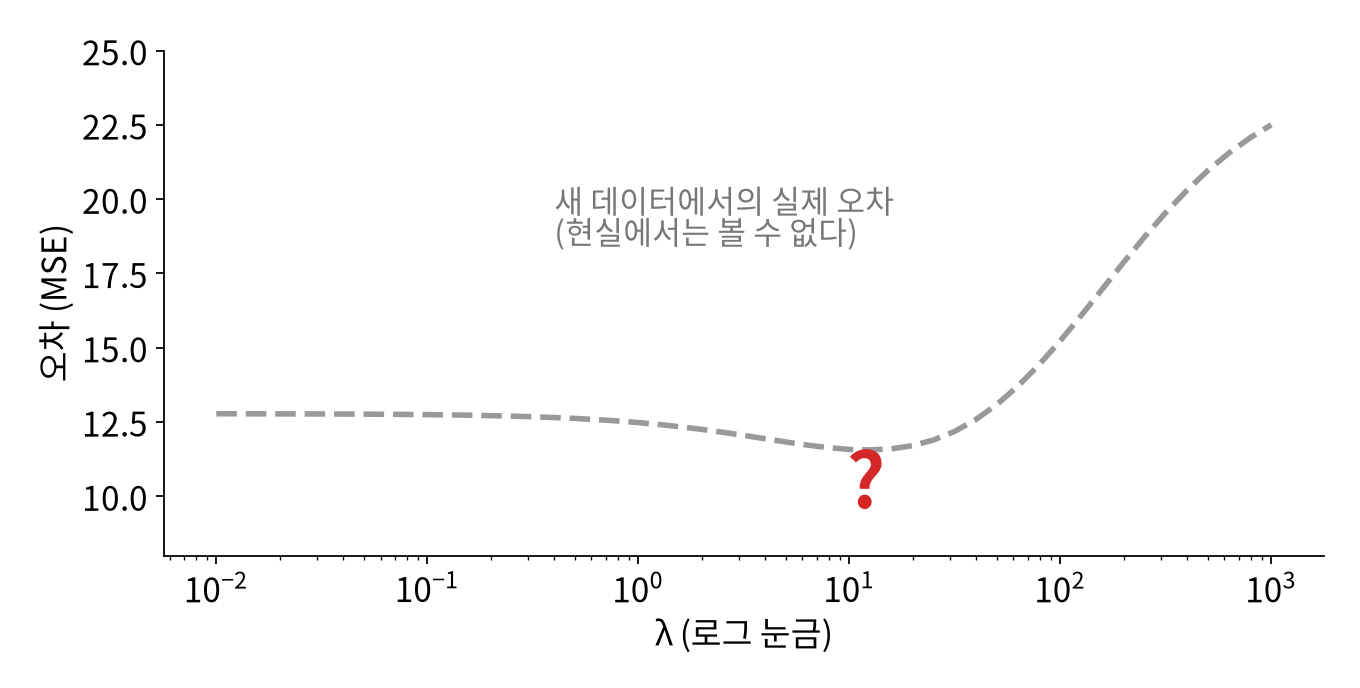
\includegraphics[width=0.62\linewidth]{cv_hook.png}\par\vskip0.2em
{\large $\lambda$ 에 따른 오차는 U 자. \kq{그런데 현실에서는 이 곡선이 안 보인다.}}
\vfill
\note{지난 시간 정규화에서 람다를 바꾸면 새 데이터 오차가 U자를 그린다는 걸 봤습니다. 그때는 예시 데이터라서 정답 곡선을 알았습니다. 하지만 현실에서는 새 데이터가 아직 없으니 이 곡선이 보이지 않습니다. 오늘은 가진 데이터만으로 이 바닥, 가장 좋은 람다를 찾는 방법을 배웁니다. 3주차에 과대적합을 배우며 잠깐 본 교차 검증을 오늘 제대로 다룹니다.}
\end{frame}

\section{한 번 나누기}
% --- 예시
\begin{frame}{오늘의 예시: 학생 60명, 특징 30개}
\vfill
\centering
{\Large\[ y = 3x_1 - 2x_2 + 1.5x_3 + \text{noise} \qquad (x_4 \sim x_{30}: \text{쓸모없는 특징 27개}) \]}\vskip0.6em
{\large 특징 30개에 데이터 60개 \quad $\to$ \quad 그냥 맞추면 잡음을 외우기 쉽다 \quad $\to$ \textbf{릿지}}\\[0.6em]
{\large 후보 $\lambda$ 51개 ($0.01 \sim 1000$, 로그 간격) 중 하나를 골라야 한다}\\[0.4em]
{\small 예시라서 새 데이터 2만 개로 ``실제 오차''를 잴 수 있다 (채점용, 고를 때는 안 쓴다)}
\vfill
\note{오늘의 예시입니다. 학생 60명에게 특징 30개가 있는데, 실제로 y를 만드는 건 그중 3개뿐이고 나머지 27개는 쓸모없는 특징입니다. 특징 30개에 데이터 60개면 그냥 선형회귀를 하면 잡음을 외우기 쉽습니다. 그래서 릿지를 쓰는데, 람다 후보 51개 중 하나를 골라야 합니다. 예시 데이터라서 같은 규칙으로 새 데이터 2만 개를 만들어 실제 오차를 잴 수 있습니다. 이건 우리 방법이 맞는지 채점하는 데만 쓰고, 고를 때는 절대 쓰지 않습니다.}
\end{frame}

% --- 한 번만 나누면
\begin{frame}{검증 데이터를 한 번만 떼어 두면}
\markpage{single}
\vfill
\centering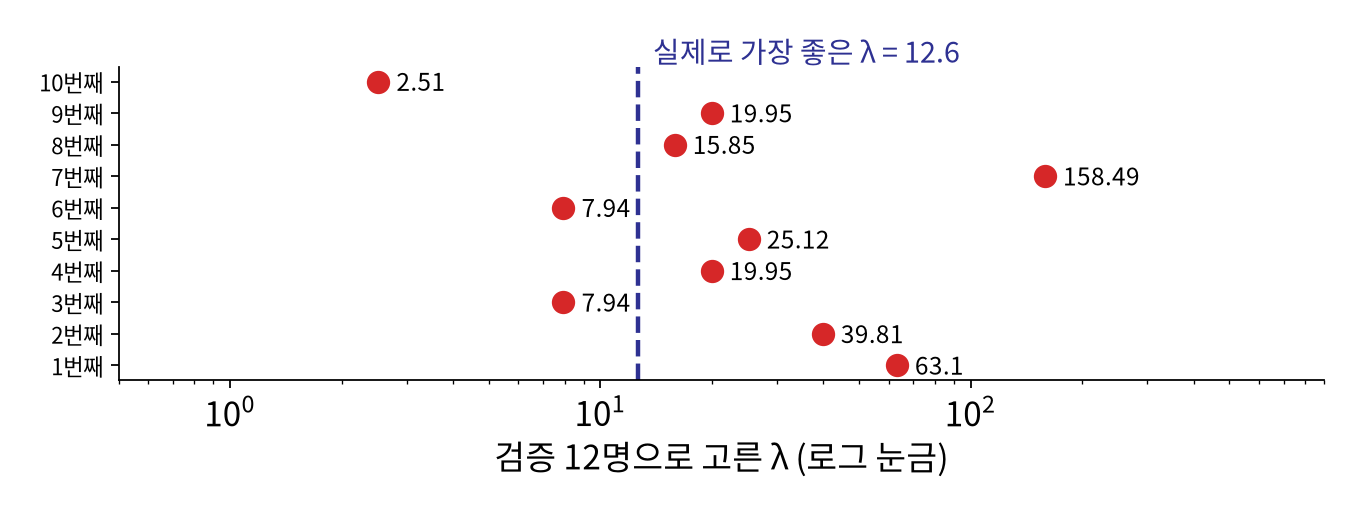
\includegraphics[width=0.66\linewidth]{cv_single.png}\par\vskip0.2em
{\large 학습 48 · 검증 12 로 \textbf{무작위로} 10번 나누면 \quad 고른 $\lambda$: \kq{2.5 $\sim$ 158}}\\[0.2em]
{\small 검증 12명이 누구냐에 따라 답이 60배 넘게 달라진다 $\to$ 한 번의 분할은 운이다}
\vfill
\note{가장 간단한 방법은 검증 데이터를 한 번 떼어 두는 겁니다. 60명 중 12명을 숨기고 48명으로 람다마다 학습한 뒤, 숨긴 12명에서 가장 잘 맞는 람다를 고릅니다. 그런데 어느 12명을 숨기느냐에 따라 결과가 크게 달라집니다. 무작위로 10번 나눠 봤더니 고른 람다가 2.5부터 158까지, 60배 넘게 흩어졌습니다. 실제로 가장 좋은 람다는 파란 선 12.6입니다. 12명은 너무 적어서 그 12명이 우연히 어떤 학생들이냐가 답을 좌우합니다.}
\end{frame}

\section{k겹}
% --- k-fold
\begin{frame}{$k$ 겹 교차 검증: 모두가 한 번씩 검증 데이터}
\markpage{kfold}
\vfill
\centering
{\LARGE\[ \text{CV}(\lambda) = \frac{1}{k}\sum_{j=1}^{k} \text{MSE}_j(\lambda) \]}\vskip0.4em
\renewcommand{\arraystretch}{1.3}
{\large\begin{tabular}{rl}
1 & 데이터를 $k$ 조각으로 나눈다 (오늘은 $k = 5$, 한 조각 12명)\\
2 & 조각 $j$ 를 숨기고 나머지 48명으로 학습 $\to$ 숨긴 12명의 MSE$_j$\\
3 & $j = 1, \dots, k$ 반복해서 평균 \quad $\to$ 모든 학생이 정확히 한 번 검증에 쓰인다\\
4 & $\lambda$ 후보마다 1$\sim$3 을 하고, $\text{CV}(\lambda)$ 가 가장 작은 $\lambda^*$ 를 고른다
\end{tabular}}
\vfill
\note{해결책은 돌아가며 숨기는 겁니다. 60명을 12명씩 5조각으로 나누고, 첫 조각을 숨기고 나머지 48명으로 학습해서 숨긴 12명의 오차를 잽니다. 다음엔 둘째 조각을 숨기고, 이렇게 다섯 번 하면 모든 학생이 정확히 한 번씩 검증 데이터가 됩니다. 다섯 오차의 평균이 교차 검증 오차입니다. 람다 후보 51개마다 이걸 하고, 교차 검증 오차가 가장 작은 람다를 고릅니다. 학습은 51 곱하기 5, 255번 합니다.}
\end{frame}

% --- 손으로
\begin{frame}{손으로 한 번: 평균만 내는 모델}
\markpage{hand}
\vfill
\centering
{\large 데이터 $y = 1, 2, \dots, 10$ \quad 모델: 학습 데이터의 \textbf{평균}으로 예측 \quad 순서대로 2개씩 5조각}\vskip0.5em
\renewcommand{\arraystretch}{1.25}
{\large\begin{tabular}{cccc}
조각 & 검증 & 학습 8개의 평균 & MSE\\\hline
1 & 1, 2 & 6.5 & $\frac{(1-6.5)^2 + (2-6.5)^2}{2} = 25.25$\\
2 & 3, 4 & 6.0 & 6.50\\
3 & 5, 6 & 5.5 & 0.25\\
4 & 7, 8 & 5.0 & 6.50\\
5 & 9, 10 & 4.5 & 25.25
\end{tabular}}\vskip0.4em
{\large CV $= \dfrac{25.25 + 6.5 + 0.25 + 6.5 + 25.25}{5} = \kb{12.75}$ \qquad 조각마다 크게 다르다}
\vfill
\note{손으로 한 번 해 봅니다. 데이터는 1부터 10까지, 모델은 아주 단순하게 학습 데이터의 평균으로 예측합니다. 첫 조각은 1과 2를 숨기고, 나머지 3부터 10까지의 평균 6.5로 예측합니다. 오차 제곱은 30.25와 20.25, 평균 25.25입니다. 같은 식으로 다섯 조각을 하면 25.25, 6.5, 0.25, 6.5, 25.25이고 평균 12.75입니다. 조각마다 오차가 0.25부터 25.25까지 크게 다르다는 점을 기억하세요. 그래서 여러 조각을 평균 내는 겁니다. 참고로 진짜 평균 5.5로 예측했을 때의 오차는 8.25인데, 교차 검증은 8개만으로 학습하니 그보다 조금 비관적으로 나옵니다.}
\end{frame}

% --- 곡선
\begin{frame}{5겹 교차 검증으로 고른 $\lambda$}
\markpage{curve}
\vfill
\centering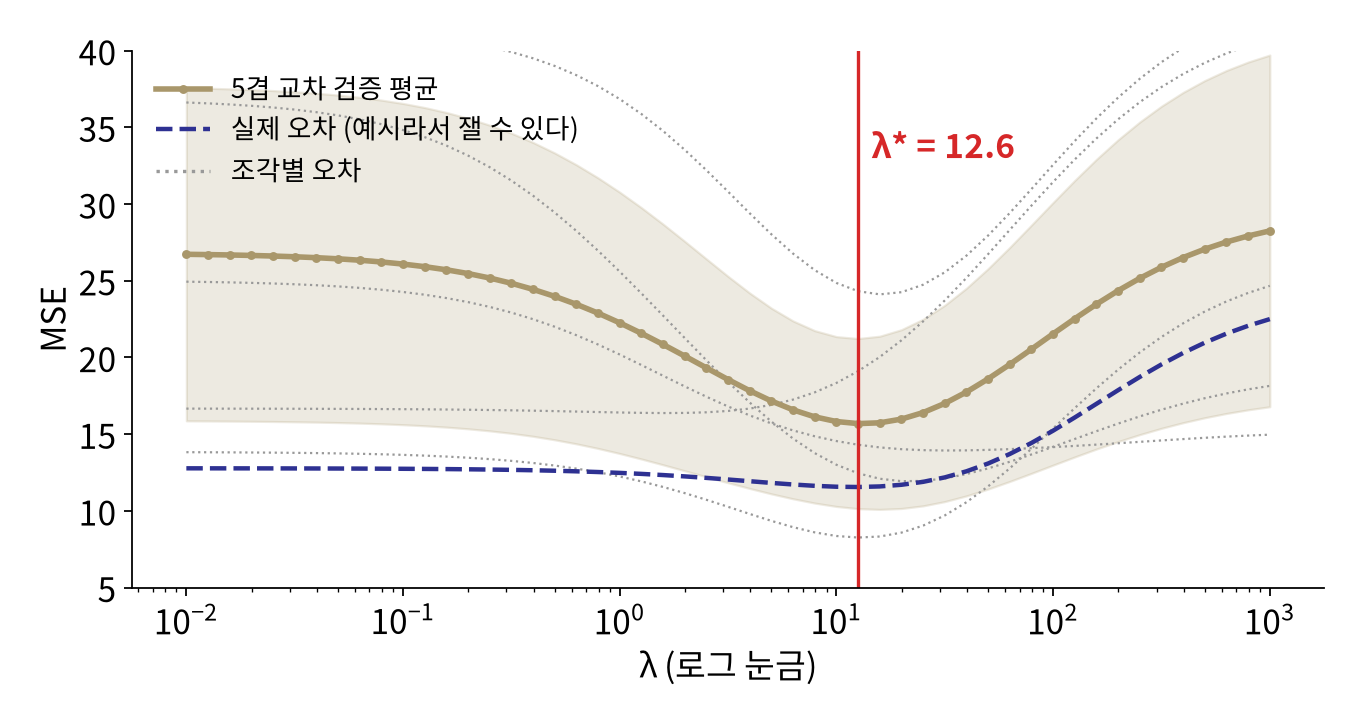
\includegraphics[width=0.64\linewidth]{cv_curve.png}\par\vskip0.2em
{\large 교차 검증 바닥 $\lambda^* = \kb{12.6}$ \quad = 실제 오차가 가장 작은 $\lambda$ (11.56)}\\[0.2em]
{\small $\lambda = 0.01$: 실제 12.78 \quad $\lambda = 1000$: 22.5 \quad 높이는 달라도 \textbf{바닥 위치}를 맞힌다}
\vfill
\note{5겹 교차 검증 결과입니다. 노란 선이 교차 검증 평균, 회색 점선이 조각별 오차, 띠는 조각 사이의 흩어짐입니다. 바닥은 람다 12.6입니다. 파란 점선은 채점용 실제 오차인데, 이것도 람다 12.6에서 가장 작습니다. 교차 검증은 새 데이터를 하나도 쓰지 않고 실제로 가장 좋은 람다를 찾아냈습니다. 교차 검증 곡선은 실제 곡선보다 위에 있습니다. 48명으로만 학습하니 조금 비관적입니다. 높이는 달라도 바닥 위치를 맞히면 고르는 데는 충분합니다.}
\end{frame}

% --- 조각별 흩어짐
\begin{frame}{바닥에서도 조각마다 다르다}
\vfill
\centering
{\Large $\lambda^* = 12.6$ 에서 조각 5개의 MSE: \quad 19.1, \; 8.3, \; 12.4, \; 24.3, \; 14.3}\\[0.8em]
{\Large 평균 \kb{15.69} \quad 표준편차 \kq{5.54}}\\[1.0em]
{\large 바닥 근처 $\lambda$ 끼리의 차이 < 조각 사이 흩어짐 \quad $\to$ \textbf{그 근처 범위}가 다 괜찮다}\\[0.4em]
{\small 1SE 규칙: 바닥 + 표준편차 1개 안에서 가장 큰 $\lambda$ (79.4, 실제 오차 14.4) $\to$ 더 단순, 조금 손해}
\vfill
\note{바닥 람다 12.6에서도 다섯 조각의 오차는 8.3부터 24.3까지 흩어져 있습니다. 평균 15.69, 표준편차 5.54입니다. 바닥 근처의 람다 몇 개는 평균 차이가 이 흩어짐보다 훨씬 작습니다. 그러니 정확히 12.6이 최고라기보다 그 근처가 다 괜찮다고 읽어야 합니다. 그래서 일부러 더 단순한, 즉 람다가 큰 모델을 고르는 규칙도 있습니다. 바닥 오차에 표준편차 하나를 더한 값 안에서 가장 큰 람다를 고르는 1SE 규칙입니다. 이 예에서는 79.4까지 허용되는데, 실제 오차는 14.4로 조금 나빠집니다. 단순함과 정확도를 바꾸는 선택입니다.}
\end{frame}

% --- 데이터가 바뀌면
\begin{frame}{데이터를 새로 뽑으면 $\lambda^*$ 도 흔들린다}
\vfill
\centering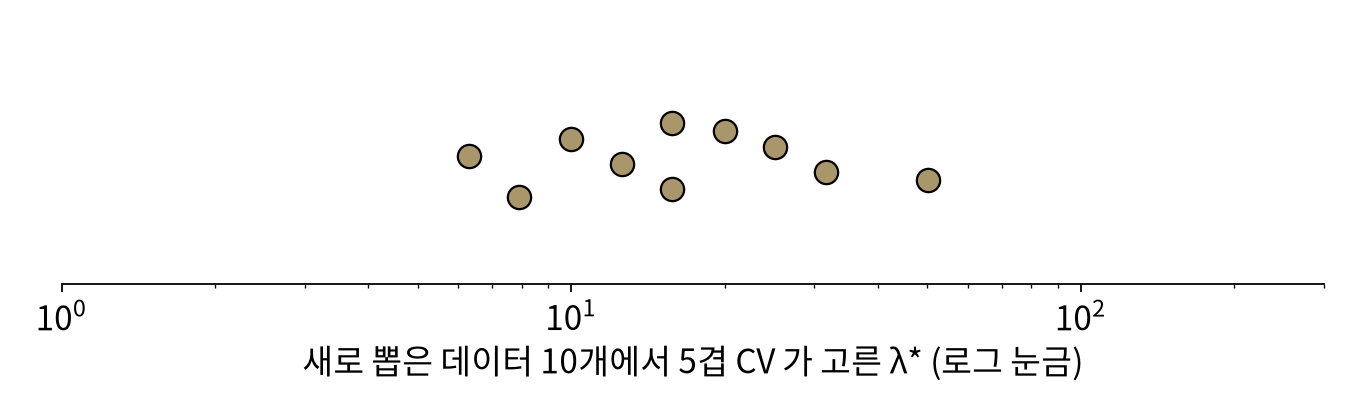
\includegraphics[width=0.66\linewidth]{cv_seeds.png}\par\vskip0.2em
{\large 같은 규칙으로 60명을 10번 새로 뽑으면 $\lambda^*$: \kb{6.3 $\sim$ 50}}\\[0.2em]
{\small 한 번 나눌 때 (2.5 $\sim$ 158) 보다 훨씬 좁다. 하지만 $\lambda^*$ 도 데이터에서 나온 \textbf{추정값}이다}
\vfill
\note{같은 규칙으로 학생 60명을 10번 새로 뽑아서 매번 5겹 교차 검증을 했습니다. 고른 람다는 6.3부터 50 사이입니다. 한 번만 나눴을 때 2.5부터 158까지 흩어졌던 것보다 훨씬 안정적입니다. 그래도 흩어지기는 합니다. 람다 별표도 결국 데이터에서 나온 추정값이라는 뜻입니다. 데이터가 많아질수록 이 흩어짐은 줄어듭니다.}
\end{frame}

\section{주의}
% --- k 는 몇
\begin{frame}{$k$ 는 몇으로?}
\vfill
\centering
\renewcommand{\arraystretch}{1.5}
{\large\begin{tabular}{lll}
$k$ & 한 번 학습에 쓰는 비율 & 특징\\\hline
2 & 50\% & 빠르지만 오차를 크게 본다\\
\textbf{5, 10} & 80\%, 90\% & \kb{가장 흔한 선택}\\
$m$ (leave-one-out) & $m - 1$ 개 & 학습 $m$ 번, 데이터가 아주 적을 때
\end{tabular}}\vskip1.0em
{\large 학습 횟수 $= k \times$ (후보 수) \quad 오늘: $5 \times 51 = 255$ 번}
\vfill
\note{k는 몇으로 할까요? k가 2면 절반으로만 학습하니 빠르지만 오차를 실제보다 크게 봅니다. k를 키울수록 학습 데이터가 많아져 실제 상황에 가까워지지만, 학습을 그만큼 여러 번 해야 합니다. 가장 흔한 선택은 5나 10입니다. k를 데이터 수와 같게 하면 하나씩 빼는 leave-one-out이고, 데이터가 아주 적을 때 씁니다. kNN 시간에 과일 21개로 써 봤습니다. 비용은 k 곱하기 후보 수만큼 학습하는 것이라, 오늘은 255번 학습했습니다.}
\end{frame}

% --- 흔한 실수: 정렬
\begin{frame}{흔한 실수: 정렬된 데이터를 섞지 않고 자르기}
\markpage{sorted}
\vfill
\centering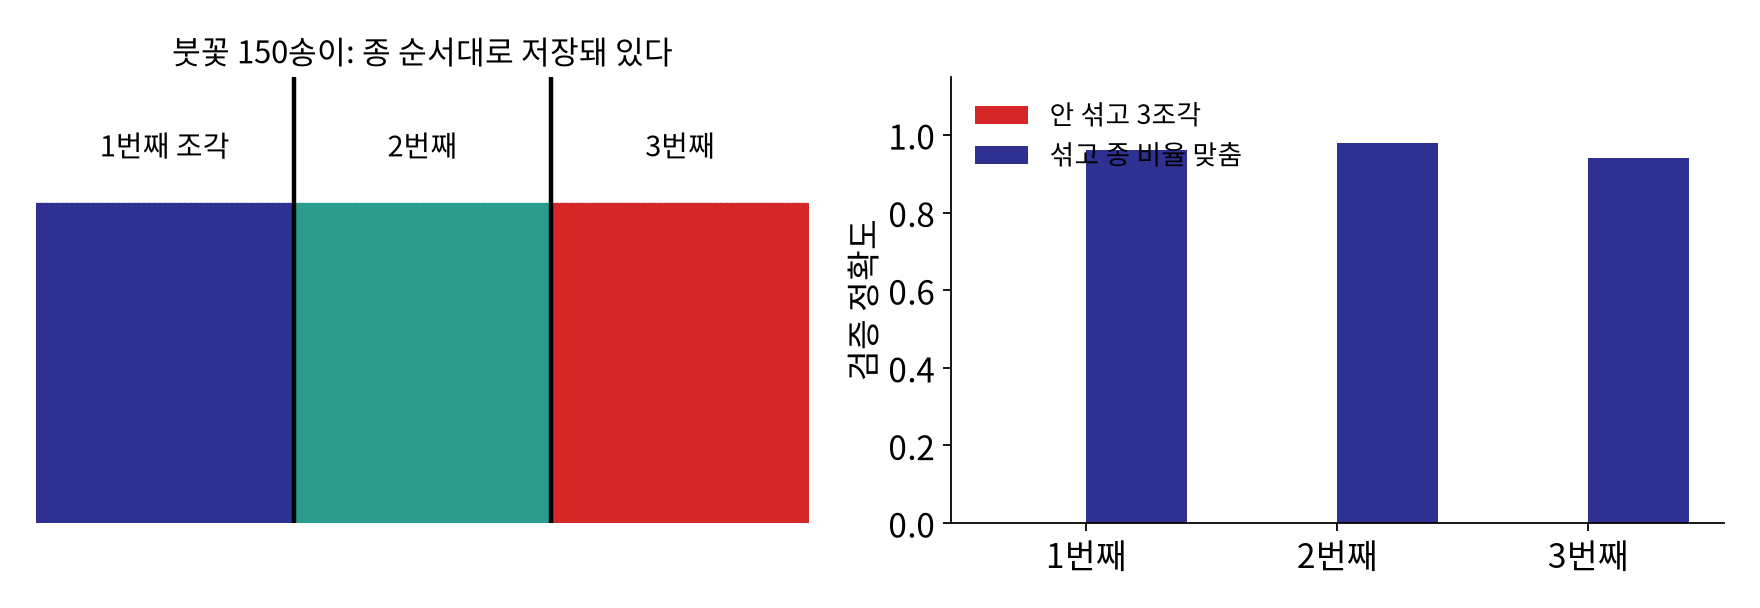
\includegraphics[width=0.86\linewidth]{cv_sorted.png}\par\vskip0.2em
{\large 종 순서대로 저장된 붓꽃을 안 섞고 3조각 $\to$ 검증 정확도 \kq{0, 0, 0}}\\[0.2em]
{\small 학습에 없던 종만 검증에 나온다. 섞고 종 비율을 맞추면 (stratified) 0.96 · 0.98 · 0.94}
\vfill
\note{교차 검증에서 가장 흔한 실수입니다. 붓꽃 데이터 150송이는 첫 50송이가 setosa, 다음 50송이가 versicolor, 마지막 50송이가 virginica로 종 순서대로 저장돼 있습니다. 이걸 섞지 않고 3조각으로 자르면, 첫 조각을 검증할 때 학습 데이터에는 setosa가 하나도 없습니다. 본 적 없는 종을 맞힐 수는 없으니 정확도가 0, 0, 0입니다. 섞고, 조각마다 종 비율까지 맞추면 0.96, 0.98, 0.94가 나옵니다. 조각마다 종 비율을 맞추는 것을 stratified, 층화라고 합니다. scikit-learn의 KFold는 기본이 섞지 않는다는 점을 꼭 기억하세요.}
\end{frame}

% --- 고른 뒤
\begin{frame}{고른 다음에: 최종 성능은 따로 잰다}
\vfill
\centering
\renewcommand{\arraystretch}{1.5}
{\large\begin{tabular}{rl}
1 & 교차 검증으로 $\lambda^*$ 를 고른다\\
2 & 가진 데이터 \textbf{전부}로 $\lambda^*$ 모델을 다시 학습한다\\
3 & 최종 성능은 \kq{한 번도 안 쓴 시험 데이터}로 잰다
\end{tabular}}\vskip1.0em
{\large 고를 때 쓴 교차 검증 점수는 \kq{조금 낙관적} (51개 중 가장 운 좋은 것)}\\[0.4em]
{\small $\to$ 다음 시간: train / val / test 분리와 데이터 누수}
\vfill
\note{람다를 골랐으면 어떻게 할까요? 가진 데이터 전부로 그 람다의 모델을 다시 학습합니다. 교차 검증 중에는 48명으로만 학습했으니까요. 그리고 최종 성능은 지금까지 한 번도 쓰지 않은 시험 데이터로 잽니다. 고를 때 쓴 교차 검증 점수를 그대로 최종 성능이라고 보고하면 안 됩니다. 후보 51개 중 가장 잘 나온 것을 골랐으니, 그 점수에는 운이 조금 섞여서 낙관적입니다. 이 이야기는 다음 시간 train, val, test 분리와 데이터 누수에서 자세히 합니다.}
\end{frame}

\section{연습}
% --- 문제풀이
\begin{frame}{문제풀이}
\vfill
\begin{enumerate}
\item 데이터 $y = 2, 4, 6, 8$, 평균 모델, 순서대로 2조각 (2겹). 조각별 MSE 와 CV 는?\vskip0.8em
\item 데이터 1,000개, $\lambda$ 후보 20개, 10겹 교차 검증. 모델을 모두 몇 번 학습하나? 마지막 재학습까지 치면?\vskip0.8em
\item 날짜 순으로 정렬된 주가 데이터에 섞어서 5겹 교차 검증을 했더니 정확도가 아주 높았다. 무엇이 의심스러운가?\vskip0.8em
\item 교차 검증 평균 오차가 $\lambda = 1$ 에서 10.0 (표준편차 2.0), $\lambda = 10$ 에서 10.5 였다. 어느 쪽을 고르겠나?
\end{enumerate}
\vfill
\note{1번 답. 첫 조각은 2와 4를 숨기고 6과 8의 평균 7로 예측하니 25와 9, MSE 17입니다. 둘째 조각은 6과 8을 숨기고 평균 3으로 예측하니 9와 25, MSE 17입니다. CV는 17입니다. 2번 답. 20 곱하기 10, 200번이고 마지막 재학습까지 201번입니다. 3번 답. 시간 순서가 있는 데이터를 섞으면 미래 데이터로 학습해서 과거를 맞히는 셈이라 성능이 부풀어 오릅니다. 다음 시간에 다룹니다. 4번 답. 차이 0.5가 표준편차 2.0보다 훨씬 작으니 둘은 사실상 같습니다. 더 단순한, 즉 정규화가 더 센 람다 10을 고르는 것도 합리적입니다.}
\end{frame}

% --- 실습
\begin{frame}{실습}
\vfill
\centering\begin{tabular}{rl}
\large 1 & $k$ 겹 교차 검증 직접 구현 $\to$ 손 계산 12.75 와 $\lambda^* = 12.6$ 재현\\[0.5em]
\large 2 & 한 번 나누기 vs 5겹: 고른 $\lambda$ 가 얼마나 흔들리나\\[0.5em]
\large 3 & 실제 데이터: 붓꽃 (안 섞으면 0\%), 당뇨병 \texttt{LassoCV} 로 $\lambda$ 고르기
\end{tabular}\vskip1em
Iris (Fisher, 1936) · Diabetes (Efron et al., 2004) \\[0.4em]\href{https://colab.research.google.com/github/SuminHan/book-ml/blob/main/slides/v2/ml1/week06/cross_validation/lab/cross_validation.ipynb}{\textcolor{ksagolddk}{▶ Colab에서 실습 노트북 열기}}
\vfill
\note{실습은 세 부분입니다. 첫째, k겹 교차 검증을 직접 구현해서 손 계산 12.75와 람다 12.6을 재현합니다. 둘째, 한 번 나누기와 5겹 교차 검증이 고르는 람다가 얼마나 흔들리는지 직접 비교합니다. 셋째, 붓꽃 데이터로 섞지 않을 때의 함정을 확인하고, 당뇨병 데이터에서 scikit-learn의 LassoCV로 람다를 고릅니다.}
\end{frame}

\section{정리}
% --- 정리
\begin{frame}{정리}
\vfill
\centering\large\begin{tabular}{l}
검증 데이터를 한 번만 떼면 \kq{운}에 좌우된다 ($\lambda$: 2.5 $\sim$ 158)\\[0.5em]
\textbf{$k$ 겹 교차 검증} \quad 돌아가며 숨기고 평균 \quad $\to$ 바닥 $\lambda^* = 12.6$ (실제로도 최선)\\[0.5em]
조각마다 흩어짐이 있다 $\to$ 바닥 근처는 다 괜찮다 (1SE 규칙)\\[0.5em]
\textbf{섞어서} 자르고, 고른 뒤 최종 성능은 \kq{시험 데이터}로
\end{tabular}
\vfill
\note{정리합니다. 검증 데이터를 한 번만 떼어 두면 어느 데이터가 뽑혔느냐는 운에 좌우됩니다. k겹 교차 검증은 돌아가며 숨기고 평균을 내서, 오늘 예시에서 실제로도 가장 좋은 람다 12.6을 찾아냈습니다. 조각마다 오차가 흩어지니 바닥 근처는 다 괜찮다고 보고, 단순함을 원하면 1SE 규칙을 씁니다. 데이터는 꼭 섞어서 자르고, 고른 뒤의 최종 성능은 따로 떼어 둔 시험 데이터로 잽니다.}
\end{frame}
\end{document}
